\documentclass[english, no-theorem-numbers]{short-notes}

\usepackage{math-alg,math-ag}

\addbibresource{math.bib}
%\bibliography{math.bib}

\title{Spectral geometry of Hecke algebras and traces}
\author{David Nadler\\ Lecture notes by Clemens Koppensteiner}
\date{July 1--8, 2013}
\version{0}

\begin{document}

\maketitle

\tableofcontents
\bigskip\noindent
By geometry we mean that we work in the function field case, with a base field $k$ of characteristic $0$.

\section{Derived algebraic geometry}

While algebraic geometers ostensibly study solutions to polynomial equations, it has been long known that it is important to keep track of the actual equations instead of merely their solutions.
Hence we can say that Algebraic Geometry is the study of \emph{systems} of polynomial equations.
An example of our slogan \enquote{equations over solutions} is the importance of nilpotents.

General references for this section are the works of Toën-Vezzosi and Lurie.

\subsection{Three examples of \enquote{derived equations}}

\subsubsection{Intersection multiplicities}

Consider $\as 4 = \Spec k[x,y,z,w]$ and the subvarieties $X₁ = \{x = y = 0\} \cup \{z=w=0\} = \{xz=xw=yz=yw\}$ and $X₂ = \{x = z,\, y = w\}$.
Obviously, $X₁ \cap X₂ = \{0\}$.
However, if we perturb $X₂$ by a little bit, we get two points.

If we impose all equations for $X₁\cap X₂$, then we get $x² = xy = xy = y²$.
Note that we get $xy$ in two different ways: from $xw = 0$, $y = w$ and from $yz = 0$, $x = z$.
Thus the dimension of $\O_{X₁ \cap X₂}$ is $3$ instead of the expected $2$ in the perturbed, \enquote{transversal} situation.
Serre's intersection multiplicity formula tells us that 
\[ 2 = 3 - 1, \]
where the $1$ is the dimension of a $\Tor$.

\subsubsection{Base change}

Consider a Cartesian diagram
\[
    \begin{tikzpicture}
        \matrix[commutative diagram] (m) {
            X₁ ×_Y X₂ & X₂ \\
            X₁ & Y \\
        };
        \path[commutative diagram arrows]
            (m-1-1) edge node[above] {$p₂$} (m-1-2)
                    edge node[left] {$p₁$} (m-2-1)
            (m-1-2) edge node[right] {$f₂$} (m-2-2)
            (m-2-1) edge node[below] {$f₂$} (m-2-2);
    \end{tikzpicture}
\]
Base change is the statement that ${p₂}_*p₁^* = f₂^*{f₁}_*$ as functors $\catCoh{X₁} → \catCoh{X₂}$.
Here and in the rest of the document all categories of modules and all functors between them are automatically derived, even when not explicitly mentioned in the notation.

Unfortunately, base change fails even in simple situations.
\begin{Ex}
    Consider the diagram 
    \[
        \begin{tikzpicture}
            \matrix[commutative diagram] (m) {
                \{0\} ×_{\as 1} \{0\} & \{0\} \\
                \{0\} & \as 1 \\
            };
            \path[commutative diagram arrows]
            (m-1-1) edge (m-1-2)
                    edge (m-2-1)
            (m-1-2) edge (m-2-2)
            (m-2-1) edge (m-2-2);
        \end{tikzpicture}
    \]
    Classically, the upper left corner is simply equal to $\{0\}$ again.
    The functor $\catModules{k} → \catModules{k}$ around the upper left part of the diagram is simply the identity, while the functor around the lower right is given by tensoring with the complex $k[1]\oplus k$.
    Derived algebraic geometry will change the upper functor ($\id$ in this case) by changing the fiber product.
\end{Ex}

\begin{Exercise}
    Let $Q^3 = \{A ∈ M₂ : \det A = 0\}$.
    This has two canonical resolutions $Q^3_+$ and $Q³_-$ given by adding a line in the kernel or cokernel of the matrix (they are a basic example of a \enquote{flop}).
    Find the correct (derived) fiber product $\tilde Q = Q³_+ ×_{Q³} Q³_-$, so that base change holds.
    (You will need material discussed later in this section to do the exercise.)
\end{Exercise}

\subsubsection{Moduli problems}

Classically there are strange ambiguities, in particular for deformations.

\begin{Ex}
    Let $\mathcal M_n$ be the moduli space of two commuting operators on $k^n$.
    We can write $\mathcal M_n$ as a fiber product
    \[
        \begin{tikzpicture}
            \matrix[commutative diagram] (m) {
                \mathcal M_n & M_n^2 \\
                \{0\} & M_n \\
            };
            \path[commutative diagram arrows]
            (m-1-1) edge (m-1-2)
                    edge (m-2-1)
            (m-1-2) edge node[right] {$[\,{,}\,]$} (m-2-2)
            (m-2-1) edge (m-2-2);
        \end{tikzpicture}
    \]
    For $n = 1$ we obtain
    \[
        \begin{tikzpicture}
            \matrix[commutative diagram] (m) {
                \mathcal M₁ & \as 1 × \as 1 \\
                \{0\} & M₁ \\
            };
            \path[commutative diagram arrows]
            (m-1-1) edge (m-1-2)
                    edge (m-2-1)
            (m-1-2) edge node[right] {$[\,{,}\,]$} (m-2-2)
            (m-2-1) edge (m-2-2);
        \end{tikzpicture}
    \]
    and, since any two matrices in $M₁$ commute, that $\mathcal M₁ = \as 1 × \as 1$.
    But if we deform slightly and require that $[\,{,}\,] = λ \ne 0$, then the moduli space suddenly becomes empty!
\end{Ex}

\subsection{Local (affine) DAG}

Imposing equations translates to tensor products and in a derived setting this means that we have to keep track of $\Tor$s.

\begin{Def}
    A \emph{commutative differential-graded algebra} (\emph{cdga}) $A^\cx$ over $tk$ is a commutative, associative algebra in $k$-chain complexes.
\end{Def}

\begin{Rem}
    We consider cdgas only up to quasi-isomorphism, but be aware that $A^\cx$ knows more that $H^\cx(A^\cx)$.
\end{Rem}

\begin{Exercise}
    Give an example of two cdgas with the same cohomology algebra (hint: Massey products).
\end{Exercise}

\begin{Def}
    A \emph{derived ring} $A^\cx$ is a cdga which is connective, i.e.~$H^iA^\cx = 0$ for $i > 0$.
    The opposite category to derived rings is called the category of \emph{affine derived schemes}.
\end{Def}

\begin{Notation}
    We often write $π_i = H^{-i}$.
\end{Notation}

\begin{Rem}
    We have a canonical map $A^\cx → π₀A^\cx$.
    Hence we can view $A^\cx$ as a \enquote{derived thickening} of $π₀A^\cx$.
    On schemes, we see this as an embedding $\Spec π₀A^\cx \hookrightarrow \Spec A^\cx$.
\end{Rem}

The source of all examples for derived rings are iterated fiber products where we keep track of $\Tor$ complexes.

\subsubsection{Structure of cdgas}

The category of cdgas should be properly viewed as an $∞$-category and is a simplicial localization of a model category.
The main structure are simplicial sets of $\Hom$:
\[
    \Hom^n(A,B) = \Hom^0(A, B \otimes Ω^\cx(Δ^n)).
\]
Practically, to calculate derived operations we only need to know the following:
\begin{enumerate}
    \item All objects are fibrant.
    \item Cell cdgas are cofibrant.
\end{enumerate}

\begin{Def}
    A cdga $A$ is a \emph{cell cdga} if it has a filtration
    \[
        k = A_0 \hookrightarrow A₁ \hookrightarrow A₂ \hookrightarrow \dotsb \hookrightarrow A_n = A,
    \]
    such that $A_{i+1} = A_i[x_i]$ with $\deg x_i ∈ ℤ$ and $dx_i ∈ A_i$.
    \todo{Is this the same as semifree algebras?}%
    \todo{Rather than $k$ should we start with the algebra over which we are taking the tensor product?}%
\end{Def}

\begin{Ex}
    Consider a hypersurface $X = \{f = 0\}$ in $\as n$.
    Traditionally we have $\O(X) = \rquot{k[x₁,\dotsc,x_n]}{(f)}$.
    The cofibrant replacement of this is $k[x₁,\dotsc,x_n][ε]$ with $\deg ε = -1$ (and hence $ε²=0$) and $dε = f$.
\end{Ex}

\subsubsection{Linearization}

Let $A$ be a derived ring.

\paragraph{Modules}
Attached to $A$ are various categories of modules, which are summarized in Figure~\ref{fig:modules}.
\begin{figure}[htb]
    \centering
    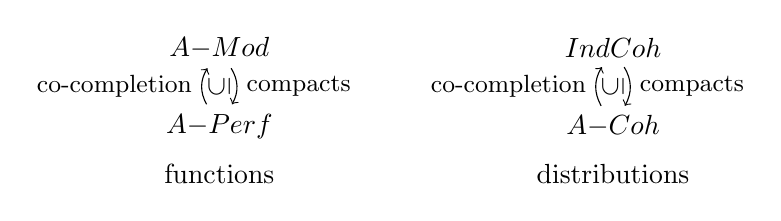
\begin{tikzpicture}
        \node (QCoh) at (0,0) {$A\text{-}\cat{Mod}$};
        \node at (0,-0.5) [rotate=90] {$\subseteq$};
        \node (Perf) at (0,-1) {$A\text{-}\cat{Perf}$};
        \draw[->] (Perf) to[bend left=30] node[left] {\small co-completion} (QCoh);
        \draw[->] (QCoh) to[bend left=30] node[right] {\small compacts} (Perf);
        \node at (0,-1.6) {\enquote{functions}};
        \begin{scope}[xshift={5cm}]
            \node (IndCoh) at (0,0) {$\cat{IndCoh}$};
            \node at (0,-0.5) [rotate=90] {$\subseteq$};
            \node (Coh) at (0,-1) {$A\text{-}\cat{Coh}$};
            \draw[->] (Coh) to[bend left=30] node[left] {\small co-completion} (IndCoh);
            \draw[->] (IndCoh) to[bend left=30] node[right] {\small compacts} (Coh);
            \node at (0,-1.6) {\enquote{distributions}};
        \end{scope}
    \end{tikzpicture}
    \caption{Categories of modules attached to a derived ring.}
    \label{fig:modules}
\end{figure}
\begin{itemize}
    \item $A\text{-}\cat{Mod}$ is the category of derived dg modules.
    \item $A\text{-}\cat{Perf}$ the subcategory consisting of summands of finite complexes of shifts of $A$.
    \item $\cat{IndCoh}$ is the category of ind-coherent modules.
    \item $A\text{-}\cat{Coh}$ is the subcategory of $A\text{-}\cat{Mod}$ consisting of complexes with bounded coherent cohomology.
\end{itemize}

\paragraph{Cotangent complex}
http://tex.stackexchange.com/questions/7556/shifting-0-0-to-new-coordinate-tikz
To $A$ we attach its \emph{cotangent complex} $\mathbb L_A ∈ A\text{-}\cat{Mod}$, which is a connective modules such that $π₀\mathbb L_A$ coincides with the cotangent bundle $Ω_{π₀A}$.
The universal characterization of the cotangent complex is 
\[
    \operatorname{Der}(A,M) = \Hom(\mathbb L_A, M).    
\]
In particular we have a \enquote{Kähler differential} $d\colon A → \mathbb L_A$.

To calculate we only need to know that $\mathbb L_A$ coincides with the cotangent bundle on smooth classical affine schemes and if $D = A \otimes_C^{\mathbb L} B$, then
\[
    \mathbb L_D = \operatorname{Cone}\left( \mathbb L_A \otimes_A D → (\mathbb L_B \otimes_B D) \oplus (\mathbb L_C \otimes_C D) \right),
\]
where the map is given by pullback.

\subsection{Global DAG}

We take the functor of points viewpoint:
\[
    \begin{tikzpicture}
        \matrix[commutative diagram] (m) {
            \cat{Aff}^{\mathrm{op}} & \cat{Sets} \\
            \cat{DAff}^{\mathrm{op}} & \cat{Spaces} = \cat{SSet} \\
        };

        \path[->] 
            (m-1-1) edge node[above] {Sch} (m-1-2)
                    edge node[auto,sloped,anchor={south}] {Stacks} (m-2-2)
            (m-2-1) edge node[below] {DStacks} (m-2-2);
        \path[right hook->]
            (m-1-1) edge (m-2-1)
            (m-1-2) edge (m-2-2);
    \end{tikzpicture}
\]
In particular, Artin derived stack are given by a diagram of the form
\[
    X \leftarrow \left(X₀ \leftleftarrows X₁\right),
\]
where $X₀$ and $X₁$ are derived schemes and the two arrows $\leftleftarrows$ are smooth maps.

\begin{Ex}\leavevmode
    \begin{enumerate}
        \item $BG \leftarrow (\mathrm{pt} \leftleftarrows G$), for $G$ a group.
        \item $M_{1,1} \leftarrow (? \leftleftarrows ?)$.
        \item $S¹ \leftarrow (\mathrm{pt} \leftleftarrows ℤ)$.
            \qedhere
    \end{enumerate}
\end{Ex}

\section{Microlocal algebraic geometry}

\section{Hecke categories}

\section{Geometric traces}

\printbibliography
\end{document}
